\subsubsection{Préparer les menus}

\noindent\textbf{Nom :} Préparer les menus \\
\textbf{ID :} UC101 \\
\textbf{Description :} Le service restauration souhaite pouvoir élaborer les menus par groupe de patient. \\
\textbf{Auteur :} Nicolas SYMPHORIEN \\
\textbf{Dates(s) :} 12/06/2017 \\
\textbf{Acteurs :} Le service restauration \\
\textbf{Pré-condition :} L'utilisateur a consulté les menus d'un groupe de patient (voir cas d'utilisation ''consulter les menus`` ).

\noindent \textbf{Scénario principal :}

\begin{enumerate}
	\item Le service restauration choisi les plat d'un jour qu'il veut élaborer.
	\item Le système affiche la composition des plat du jour choisi avec les quantités pour chaque ingrédients
	\item Le service restauration peut choisir d'élaborer les plats d'un autre jour , dans ce cas le cas d'utilisation reprend à l'étape 1, sinon le cas d'utilisation se termine.
\end{enumerate}

\noindent \textbf{Post-Conditions:} Le service restauration a élaboré tous les plats des jours qu'il souhaite.

\begin{figure}
\centering
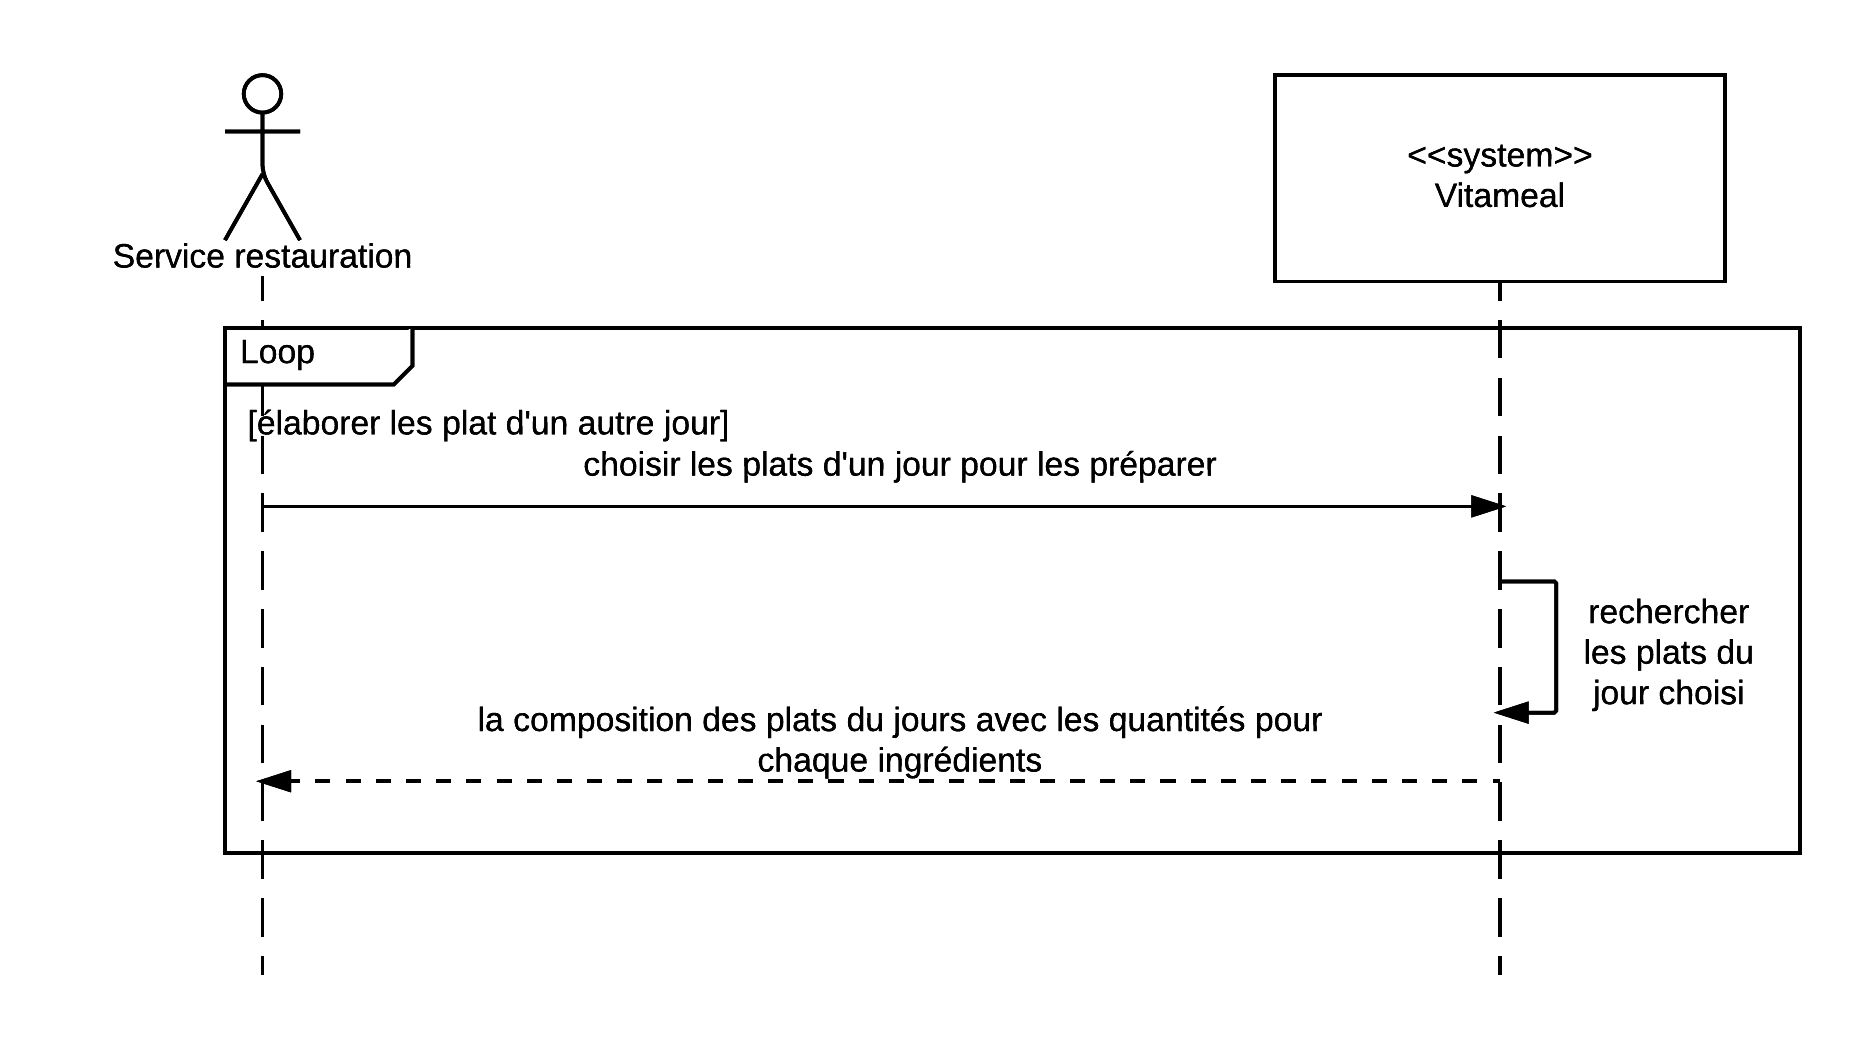
\includegraphics{../../CasDUtilisations/PreparerMenus/sequence_preparer_menus.png}
\caption{Diagramme de séquence du cas d'utilisation préparer les menus}
\end{figure}